\documentclass[12pt]{article}
\usepackage[a4paper, portrait, margin=1cm, bottom=2cm]{geometry}
\usepackage{fontspec}
\usepackage[fleqn]{amsmath}
\usepackage{amssymb}
\usepackage{graphicx}
\usepackage{indentfirst}
\usepackage{polyglossia}
\usepackage[dvipsnames]{xcolor}

\setmainfont[Ligatures=TeX]{Linux Libertine}
\setdefaultlanguage{russian}
\setotherlanguages{english}
\graphicspath{graphics}

\begin{document}

\section{Линейное пространство. Проверка на принадлежность}
\subsection{Определение}
Множество $L$ называют линейным (векторным) пространством, если на нём введены операции \textbf{ сложения} и {\bf умножения} на {\bf скаляр}, удовлетворяющие условиям:
\begin{enumerate}
    \item $x,y \in L \Rightarrow x + y \in L, $ (замкнутость)
    \item $x+y = y+x $ (коммутативность)
    \item $(x+y)+y=x+(y+z)$ (ассоциативность)
    \item $x+0=0+0$ (существование нейтрального элемента)
    \item $-x+x=0$ (существование противоположного для каждого элемента)
    \item $1 \cdot x=x \cdot 1, 1 \in F$(умножение на нейтральный скаляр по умножению не изменяет элемент)
    \item $x \in L \Rightarrow $ $\lambda x \in L$(замкнутость при умножении на скаляр)
    \item $\mathbf{\lambda} (\mathbf{\nu} x)=(\mathbf{\lambda \nu})x$(ассоциативность умножения на скаляр)
    \item $\mathbf{\alpha}(x+y)=\mathbf{\alpha}x+\mathbf{\alpha}y, \mathbf{\alpha}\in F; x \in L,y \in L;$(дистрибутивность умножения на скаляр относительно сложения векторов)
    \item $(\mathbf{\alpha}+\mathbf{\beta})x=\mathbf{\alpha}x+\mathbf{\beta}x, x \in L; \mathbf{\alpha} , \mathbf{\beta} \in F$(дистрибутивность умножения на вектор относительно сложения скаляров)

\end{enumerate}
\textbf{Примечание: L - непустое множество, элементы которого называются векторами.}\\
\textbf{F - скалярное поле. Например: $\mathbb{R}$ - множество вещественных числе, $\mathbb{C}$ - множество комплексных чисел, $\mathbb{Q}$ - множество рациональных чисел}
\subsection{Примеры векторных пространств:}
\begin{itemize}
    \item вектора в пространствах $\mathbb{R}^n, \mathbb{C}^n$
    \item матрицы m$\times$n с элементами из какого-либо поля.
    \item многочлены степени {\bf не выше} n.
\end{itemize}
\subsection{Базис}
\subsubsection{Определение}
Базис линейного простраства - линейно независимый, порождающий набор(система) векторов.\par
Линейно зависимой системой(набор) $\overrightarrow{x_1},\overrightarrow{ x_2},..,\overrightarrow{x_n}$ если существуют ненулевой набор $a_1,a_2,..,a_n$,\par что: $a_1\overrightarrow{x_1}+a_2\overrightarrow{ x_2}+..+a_n\overrightarrow{x_n}=\overrightarrow{0}$ \par Если таких коэффицентов не существует, то система линейно независимая.\\
\subsubsection{Примеры базисов:}
\begin{itemize}
    \item вектора $(1,0,0)^T,(0,1,0)^T,(0,0,1)^T$ в $\mathbb{R}^3$ или $(2,3,0)^T,(0,2,1)^T,(0,4,3)^T$, главное чтобы они были ЛНЗ .
    \item $x$, $x^2$, $x^3$ в пространстве многочленов степени меньше 3.
    \item 4 матриц с одной 1 единицей и остальными нулями в линейном пространстве матриц $2 \times 2$ с вещественными элементами:
          $\begin{pmatrix}
                  1 & 0 \\
                  0 & 0
              \end{pmatrix}$,
          $\begin{pmatrix}
                  0 & 1 \\
                  0 & 0
              \end{pmatrix}$,
          $\begin{pmatrix}
                  0 & 0 \\
                  1 & 0
              \end{pmatrix}$,
          $\begin{pmatrix}
                  0 & 0 \\
                  0 & 1
              \end{pmatrix}$.
    \item $V =\{p(t)\sin{6t}+q(t)\cos{6t} \vert deg(q(t))\leq 1, deg(p(t))\leq 1\}$ Базис: $\sin{6t},cos{6t},t\sin{6t},t\cos{6t}$.
\end{itemize}
\subsubsection{Матрица перехода}
Переход из одного базиса в другой возможен с помощью домножения на матрицу перехода A, вычисляется она по значениям на базисных векторах, ниже подробнее разобрано.\\
Пример:
\begin{itemize}
    \item {Запишите матрицу линейного оператора $L$ в базисе $u$, если известно: $L(u_1) = 2u_1 + u_2 + u_3$; $L(u_2) = u_2$;
          $L(u_3) = u_2 + u_3$.}

          \fbox{Ответ: $L_u = \begin{pmatrix}
                      2 & 0 & 0 \\
                      1 & 1 & 1 \\
                      1 & 0 & 1
                  \end{pmatrix}$}

\end{itemize}



\subsection{Проверка является ли множество векторным пространством}
Самым простым является прямое соотношение геометрическим векторам, например матрицы $2\times 2$ векторам $1\times 4$ , так как там тоже 4 упорядоченных элемента. Это делается для того, чтобы не проверять все аксиомы векторного простраства. Также доказать, что множество является векторным пространством можно, проверив все аксиомы.
\subsubsection{Примеры проверки:}
\begin{itemize}
    \item $L$ = \textbraceleft Множество многочленов степени 5\textbraceright . Не является лин. пространство, так как нет нуль-вектора, многочлен с нулевыми коэффицентами не входит в данное множество. Также нет замкнутости: $\overrightarrow{a}-\overrightarrow{a}=\overrightarrow{0} \notin L $
    \item Окружность радиуса 1 в $\mathbb{C}$ или $L = \{ \mathbb{C}  \vert  Im(z)^2+Re(z)^2 = 1 \} $. Также нет замкнутости ни при умножение на скаляр, ни при сложении.
    \item Матрицы. Не являются, так как не всегда можно складывать.

\end{itemize}

\section{Подпространство}
\subsection{Определение}
Непустое множество $L^{'} \subset L$ векторного пространства $L$ над полем $F$ является векторным подпространством, если выполнены свойства для всех элементов поля $F$ и подмножества $L^{'}$.($\subset$- обозначение подмножества):
\begin{itemize}
    \item $x+y\in L^{'} , x \in L^{'}, y \in L^{'} $
    \item $\alpha x \in L^{'}, \alpha \in F, x \in L^{'}$
\end{itemize}

\subsection{Примеры:}
\begin{itemize}
    \item Тривиальные подпространства - с одним нулевым элементов. Например матрица $\begin{pmatrix}
                  0 & 0 \\
                  0 & 0
              \end{pmatrix}$
          в векторном пространстве матриц $2\times 2$ над полем $\mathbb{R}$ или $\mathbb{C}$.
    \item тождественное подпространство $L$ для множества $L$
    \item Плоскость или прямая в $\mathbb{R}^3$ или гиперплоскость в $\mathbb{R}^n$ пространстве. Прямая и плоскость - частные случаи гиперплоскости.
    \item матрицы вида $\begin{pmatrix}
                  0 & 0 & x \\
                  0 & 0 & 0
              \end{pmatrix}$
    \item векторное пространство $ R^n[x]$ является подпространством всех многочленов $R[x]$
\end{itemize}
\subsection{Проверка является ли подпространством векторное пространство обычно сводится к проверке двух свойств, нам не нужно проверять все 10 аксиом векторного пространства: }
\begin{itemize}
    \item $x+y\in L^{'} , x \in L^{'}, y \in L^{'} $
    \item $\alpha x \in L^{'}, \alpha \in F, x \in L^{'}$

\end{itemize}
Можно заметить, что подпространство должно содержать нуль-вектор, из выше изложенных свойств.

\section{Линейный оператор.}
\subsection{Определение}
Линейным оператором называется такое отображение векторного пространства $L$ над полем $K$ в это же векторное пространство $L$ над тем же полем $f: L \longrightarrow L $, которое удовлетворяет условиям:
\begin{itemize}
    \item $f(a+b)=f(a)+f(b), \forall a \in L, \forall b \in L$
    \item $f(\alpha x)=\alpha f(x), \forall \alpha \in K, \forall x \in L$
\end{itemize}
\text{Можно заметить, что первое условие - гомоморфизм групп.}\\
\text{Также заметно важное свойство, что $\mathbf{f(\overrightarrow{0})=\overrightarrow{0}}$.}

\subsection{Способы задания линейных операторов:}
\begin{itemize}
    \item Словесный, например: проекция пространства на плоскость, проходящую в нуле,прямую, гиперплоскость.
    \item Функциональный, например: производная)
    \item Матричный ($Ax=y$, матрица $A$ умножается на вектор $x$  .
\end{itemize}
\subsection{Примеры проверки отображений :}
\begin{itemize}
    \item Проекция на плоскость $x+2y+z=3$ является линейным оператором, так как $f(\overrightarrow{0})= \overrightarrow{0}$ и $f(x+y)=f(x)+f(y)$(гомоморфизм).Аналогично с любой проекцие на плоскость и прямую
    \item $f(p(x),q(y),r(z))=(p(x)^{'},q(x)^{'},r(x)^{'})$ будет являться, а $f(p(x),q(y),r(z))=(p(x)^{'}+1,q(x)^{'}-2,r(x)^{'})$ по причине не выполнения обоих условий
    \item оператор поворота на угол $\alpha $ является линейным оператором
    \item симметрия относительно плоскости также
\end{itemize}
\subsection{Матрица линейного оператора:}
Дейсствие на вектор линейныго оператора можно представить в виде домножения на матрицу только в случае конечномерного пространства.\\
Разложим вектор x по базису. Пусть $x=a_1 e_1+a_2 e_2+..+a_n e_n$\\
Тогда $A(x)=A(a_1 e_1+ a_2 e_2+..+a_n e_n)=A(a_1 e_1)+A(a_2 e_2)+..+A(a_n e_n)=a_1 A(e_1)+a_2 A(e_2)+..+a_n A(e_n)$\\
Следовательно по значениям линейного оператора на базисе можно вычислить его значения на всём пространстве.
\subsubsection{Примеры:}
\begin{itemize}
    \item Матрица оператора дифференцирования в пространстве многочленов степени не выше 2. Базис: $e_1=1, e_2=x, e_3=x^2; A(e_1)=0, A(e_2)=1,A(e_3)=2x$. Отсюда получим матрицу оператора на базисе:
          $\begin{pmatrix}
                  0 & 1 & 0 \\
                  0 & 0 & 2 \\
                  0 & 0 & 0
              \end{pmatrix}$. Значения на базисных векторах - столбцы слева направо.
    \item Матрица оператора проекции в $\mathbb{R}^3$ на плоскость XOY:\\
          Возьмём базис $e_1=(1,0,0)^T,e_2=(0,1,0)^T,e_3=(0,0,1)^T$. \\$A(e_1)=(1,0,0)^T, A(e_2) =(0,1,0)^T, A(e_3)=(0,0,0)^T$.\\ Тогда матрица оператора A: $\begin{pmatrix}
              1 & 0 & 0 \\
              0 & 1 & 0 \\
              0 & 0 & 0
          \end{pmatrix}$
    \item Матрица поворота в $\mathbb{R}^2$:\\
          Возьмём острый угол.\\
          A$\begin{pmatrix}
                  1 \\
                  0
              \end{pmatrix}=
              \begin{pmatrix}
                  \cos{\alpha} \\
                  \sin{\alpha}
              \end{pmatrix}$,
          A$\begin{pmatrix}
                  0 \\
                  1
              \end{pmatrix}=
              \begin{pmatrix}
                  -\sin{\alpha} \\
                  \cos{\alpha}
              \end{pmatrix} \Longrightarrow A=
              \begin{pmatrix}
                  \cos{\alpha} & -\sin{\alpha} \\
                  \sin{\alpha} & \cos{\alpha}
              \end{pmatrix}$
    \item {В стандартном базисе пространства $\mathbf{R}^3$ найдите матрицу оператора $L$, если $L(v) = v - 2\dfrac{(a,v)}{(a,a)}a$, где $a = (-3, 2, 5)^T$, а $(\ ,\ )$ обозначает скалярное произведение}
          Пусть $V_1 = \begin{pmatrix} 1 \\ 0 \\ 0 \end{pmatrix}$;
          $V_2 = \begin{pmatrix} 0 \\ 1 \\ 0 \end{pmatrix}$;
          $V_3 = \begin{pmatrix} 0 \\ 0 \\ 1 \end{pmatrix}$.

          \[
              L(V_1) = \begin{pmatrix} 1 \\ 0 \\ 0 \end{pmatrix} - 2\dfrac{-3}{38}\begin{pmatrix} -3 \\ 2 \\ 5 \end{pmatrix}
              = \dfrac{1}{38}\begin{pmatrix} 20 \\ 12 \\ 30 \end{pmatrix}
              = \dfrac{1}{38}(20V_1 + 12V_2 + 30V_3)
          \]
          \[
              L(V_2) = \begin{pmatrix} 0 \\ 1 \\ 0 \end{pmatrix} - 2\dfrac{2}{38}\begin{pmatrix} -3 \\ 2 \\ 5 \end{pmatrix}
              = \dfrac{1}{38}\begin{pmatrix} 12 \\ 30 \\ -20 \end{pmatrix}
              = \dfrac{1}{38}(12V_1 + 30V_2 - 20V_3)
          \]
          \[
              L(V_3) = \begin{pmatrix} 0 \\ 0 \\ 1 \end{pmatrix} - 2\dfrac{5}{38}\begin{pmatrix} -3 \\ 2 \\ 5 \end{pmatrix}
              = \dfrac{1}{38}\begin{pmatrix} 30 \\ -20 \\ -12 \end{pmatrix}
              = \dfrac{1}{38}(30V_1 - 20V_2 - 12V_3)
          \]

          \fbox{Ответ: $L_V = \dfrac{1}{38}\begin{pmatrix}
                      20 & 12  & 30  \\
                      12 & 30  & -20 \\
                      30 & -20 & -12
                  \end{pmatrix}$}
\end{itemize}
\subsection{Матрица линейного оператора в новом базис}
Чтобы найти матрицу линейного оператора в новом базисе необходимо найти матрицу перехода в новый базис и из нового базиса в старый - обратная к первой.\\
\fbox{$L_f = T_{f\longrightarrow e} \cdot L_e \cdot T_{e\longrightarrow f}$}, \\$L_f$-матрица оператора в новом базисе\\ $T_{f\longrightarrow e}$-матрица перехода из f в e,
    \\$T_{e\longrightarrow f}$-матрица перехода из e в f

\section{Обратный оператор}
\subsection{Суть}
Обратный оператор при воздействии после воздействия изначального оператора должен вернуть тот же вектор. Обозначается $A^{-1}$.\\ Линейные операторы могут быть как \textbf{обратимыми}(переход в другой базис, симметрия), так и \textbf{необратимыми}(дифференцирование, проекция на пространство меньшей размерности).
\subsection{Способы нахождения:}
\begin{itemize}
    \item Алгебраический: нахождение обратной матрицы к матрице оператора(например методом присодинения единичной ), возможно только в конечномерном пространстве.
    \item Геометрический: Например ,если симметрия относительно плоскости, то обратный оператор будет возвращать изначальный вектор, при действии на вектор, на который прежде действовали оператором. Также Если $A$ - оператор на евклидовом пространстве $V$, то можно использовать геометрические свойства оператора для нахождения его обратного. Например, если $A$ - ортогональный оператор, то $A^{-1} = A^T$, где $A^T$ - транспонированная матрица оператора $A$
    \item Смешанный - вообще хз, Иванов даже в лс ничего не сказал
\end{itemize}

\section{Ядро и образ линейного оператора, их размерности.}
\subsection{Определение}
Пусть A - линейный оператор векторного пространства V.

Образ: множество $\forall y \in V : \exists\ x \in V : A(x) = y$. Обозначение: \emph{Im A}.

Ядро: множество $\forall x \in V : A(x) = 0$. Обозначение: \emph{Ker A}.

\subsection{Размерности Образа и Ядра}
A - линейный оператор в век. пространстве размерности n.

Размерность образа соответствует рангу матрицы оператора (Размерность $Im(A) = rk(A)$)

Размерность ядра соответствует дополнению ранга матрицы до n (Размерность $Ker(A) = n - rk(A)$)

\subsection{Доказательство подпространства}

\subsubsection{Образ}
Пусть $y_1, y_2 \in \emph{Im A}$, t - произвольное вещественное число $\Rightarrow \exists\ x_1, x_2 \in A : \begin{cases}
        A(x_1) = y_1 \\
        A(x_2) = y_2 \\
    \end{cases}
    \Rightarrow y_1 + y_2 = A(x_1)\ + A(x_2) = A(x_1 + x_2)$ и $ty_1 = tA(x_1) = A(tx_1)$ $\Rightarrow y_1 + y_2$ и ty - элементы образа $\Rightarrow$ образ - подпространство.

\subsubsection{Ядро}
Пусть $x_1, x_2 \in \emph{Ker A}$, t - произвольное вещественное число $\Rightarrow \begin{cases}
        A(x_1) = 0 \\
        A(x_2) = 0 \\
    \end{cases}
    \Rightarrow A(x_1+x_2) = A(x_1) + A(x_2) = 0 + 0 = 0, A(tx_1) = tA(x_1) = 0 \Rightarrow x_1 + x_2$ и tx - элементы ядра $\Rightarrow$ ядро - подпространство.

\subsection{Примеры}
Образ проекции пространства на плоскость $XOY$ – плоскость $XOY$, ядро этого оператора – все векторы, параллельные оси $OZ$.

Образ оператора дифференцирования на пространстве всех многочленов – это же пространство многочленов. Ядро этого оператора – константы.

\section{Алгоритм Чуркина}
\subsection{Алгоритм}
Имеется матрица оператора A размерности n. Составим матрицу B порядка n x 2n, где первые n столбцов занимает транспонированная матрица A, следующие n столбцов единичная матрица.

Элементарными преобразованиями приводим левую часть к ступенчатому виду.

Ненулевые строки левой части - базис образа оператора A.

Продолжение нулевых строк в правой части - базис ядра.

\subsection{Обоснование}
Строки $A^T$ соответствуют значению оператора на базисе.

Записав значения и приведя к ступенчатому виду, получаем базис (базис Образа).

Левая часть матрицы B соответствует значению оператора на векторе, тогда как правая - координатной записи вектора.После преобразований закономерность сохраняется и в правой части: строки соответствующие нулевым строкам в левой являются базисом ядра. (P.S. Вспомни определение ядра)

\subsection{Пример}
Пусть $A = \left(\begin{array}{cccc}
            2  & 0 & 1 & -3 \\
            1  & 0 & 3 & -4 \\
            -1 & 0 & 2 & -1 \\
            1  & 0 & 1 & -2
        \end{array} \right)$
По алгоритму:

$\left(\begin{array}{cccc|cccc}
            2  & -1 & -1 & 1  & 1 & 0 & 0 & 0 \\
            0  & 0  & 0  & 0  & 0 & 1 & 0 & 0 \\
            1  & 3  & 2  & 1  & 0 & 0 & 1 & 0 \\
            -3 & -4 & -1 & -2 & 0 & 0 & 0 & 1
        \end{array} \right)$ перемещаем строку $\left(\begin{array}{cccc|cccc}
            2  & -1 & -1 & 1  & 1 & 0 & 0 & 0 \\
            1  & 3  & 2  & 1  & 0 & 0 & 1 & 0 \\
            -3 & -4 & -1 & -2 & 0 & 0 & 0 & 1 \\
            0  & 0  & 0  & 0  & 0 & 1 & 0 & 0
        \end{array} \right)$

$l_3 \rightarrow l_3 + l_2 + l_1$ получаем $\left(\begin{array}{cccc|cccc}
            2 & -1 & -1 & 1 & 1 & 0 & 0 & 0 \\
            1 & 3  & 2  & 1 & 0 & 0 & 1 & 0 \\
            0 & 0  & 0  & 0 & 1 & 0 & 1 & 1 \\
            0 & 0  & 0  & 0 & 0 & 1 & 0 & 0
        \end{array} \right)$

Тогда: $(2,-1,-1,1), (1,3,2,1)$ - базис образа, $(1,0,1,1),(0,1,0,0)$ -базис ядра.

\section{Проверка линейного оператора на вырожденность и невырожденность}
\subsection{Невырожденная матрица оператора}
\subsection{Оператор вырожденный, если $\exists\ x_1, x_2 : A(x_1) = A(x_2) = y$. Тогда невозможно однозначно определить обратный оператор от y}
\subsection{Оператор невырожденный только тогда, когда ядро состоит только из нулевого элемента}
Оператор невырожденный $\Rightarrow$ ядро не может состоять больше чем из одного элемента (пункт 2) $\Rightarrow$ ядро состоит только из 0.

Ядро состоит из 0 $\Rightarrow A(x_1) = A(x_2)$ будет:

$A(x_1) - A(x_2) = 0 \Rightarrow A(x_1 - x_2) = 0 \Rightarrow x_1 - x_2 = 0 \Rightarrow x_1 = x_2$

Совпадение значений оператора на двух элемента $\Rightarrow$ совпадают элементы $\Rightarrow$ возможно корректное определение обратного оператора.

\subsection{Геометрические соображения}
Пример:

Вырождена ли симметрия относительно плоскости? Легко заметить, что двойная симметрия вернёт точку в исходное положение. Таким образом обратный к симметрии - это сама симметрия, а значит она невырождена.

\subsection{Примеры}
\begin{enumerate}
    \item $A(x) = a * x$, где $a \in R$.

          Ядро состоит только из нулевого элемента тогда и только тогда, когда $a \neq 0$.

          Если $a = 0$, оператор вырожден, поскольку прообраз 0 неоднозначно определён.

    \item $A(x) = (x,e)e$, при этом $|e| = 1$

          Оператор вырожден, поскольку ядро состоит не только из 0.
\end{enumerate}

\section{Собственные числа}
\subsection{Определение}
Число $\lambda$ называется собственным числом оператора $L$, если существует такой ненулевой вектор $x$, что $L(x) = \lambda x$. При этом вектор $x$ называется собственным вектором оператора $L$, отвечающим собственному числу $\lambda$.

\subsection{Вычисление}
\subsubsection{Геометрический}
Пример: Найти с.ч. и с.в. проекции пространства на плоскость $XOY$.

Найдём все векторы || своей проекции - это все вектора || $XOY$ (проекция равна вектору) и все вектора перпендикулярные плоскости (проекция равна нулю). $\Rightarrow$

$\lambda_1 = 1, X_{\lambda_1} = \left(\begin{array}{c}
            x \\
            y \\
            0
        \end{array} \right); \lambda_2 = 0, X_{\lambda_2} = \left(\begin{array}{c}
            0 \\
            0 \\
            z
        \end{array} \right)$, где $x, y, z \in R$.
\subsubsection{Аналитический}
Пример: Найти с.ч. и с.в. оператора дифференцирования на множестве всех многочленов.

Рассмотрим $p^\prime(x) = \lambda p(x)$. Если $\lambda \neq 0$, то степени правой и левой частей не совпадут. Если $\lambda = 0$, то p(x) - константа.

Ответ: $\lambda = 0, X_\lambda = C = const$.

\subsubsection{С помощью матрицы}
Пусть оператор задан матрицей $\Rightarrow A(x) = Ax \Rightarrow$

\begin{center}
    $Ax = \lambda x \Leftrightarrow Ax - \lambda x = 0 \Leftrightarrow Ax - \lambda Ex = 0 \Leftrightarrow (A - \lambda E)x = 0$
\end{center}

$\lambda$ - с.ч. только тогда, когда система уравнений на координаты x $(A - \lambda E)x = 0$ имеет ненулевое решение.

Выполняется только тогда, когда определитель $(A - \lambda E)$ равен 0.

Алгоритм: \begin{enumerate}
    \item Найти корни уравнения $det(A - \lambda E) = 0$
    \item Для каждого из корней решить СЛУ $(A - \lambda E)x = 0$. Решения будут задавать координаты множества с.в., соответствующих с.ч. (может иметь размерность 1 и более)
\end{enumerate}
\subsection{Диагонализуемость}

Если удаётся найти базис из с.в. для линейного оператора, то его матрица в этом базисе будет диагональна, а на диагонали будут с.ч.

Пусть матрица диагональна, значит элементы диагонали обозначим через $\lambda_k$ из условия $A(e_k) = \lambda_k e_k$ получим, что по определению все элементы базиса - с.в. данного линейного оператора.

Итог: матрица линейного оператора диагонализуема тогда только тогда, когда для этого линейного оператора найдётся базис из собственных векторов.

\section{Евклидовые и Унитарные пространства}
Вещественное линейное пространство $\mathbb{E}$ называется евклидовым, если каждой паре элементов $\mathbf{u},\,\mathbf{v}$ этого пространства поставлено в соответствие действительное число $\langle \mathbf{u},\mathbf{v} \rangle$, называемое скалярным произведением, причем это соответствие удовлетворяет следующим условиям:
\begin{enumerate}
    \item $(\mathbf{u},\mathbf{v})=(\mathbf{v},\mathbf{u})\ \forall\ \mathbf{u},\mathbf{v}\in \mathbb{E}$
    \item $(\mathbf{u} + \mathbf{v},\mathbf{w})=(\mathbf{u},\mathbf{w})+(\mathbf{v},\mathbf{w})\ \forall\ \mathbf{u},\mathbf{v},\mathbf{w}\in \mathbb{E}$
    \item $(k\mathbf{u},\mathbf{v})=k(\mathbf{u},\mathbf{v})\ \forall\ \mathbf{u},\mathbf{v}\in \mathbb{E},\forall k\in \mathbb{R}$
    \item $(\mathbf{u},\mathbf{u})\geq 0$ и $(\mathbf{u},\mathbf{u})=0$ только если $\mathbf{u}=\mathbf{0}$
\end{enumerate}
В скалярном произведении $\langle\mathbf{u}, \mathbf{v}\rangle$ вектор $\mathbf{u}$ — первый, а вектор $\mathbf{v}$ — второй сомножители. Скалярное произведение $\langle\mathbf{v},\mathbf{v}\rangle$ вектора $\mathbf{v}$ на себя называется скалярным квадратом. Условия 1–4 называются аксиомами скалярного произведения. Аксиома 1 определяет симметричность скалярного произведения, аксиомы 2 и 3 — аддитивность и однородность по первому сомножителю, аксиома 4 — неотрицательность скалярного квадрата $\langle\mathbf{v}, \mathbf{v}\rangle$.

\subsection{Геометрические примеры для трёхмерного евклидова пространства}

Является ли скалярным произведением:
\begin{enumerate}
    \item Смешанное произведение $(n, x, y)$, где $n$ – фиксированный вектор.

          Ответ: Нет, поскольку если $n = 0$, то $(n, x, x) = 0$ при каждом $x$, а если $n\neq 0$, то $(n, x, x) = 0$ при $x = n$.

    \item Скалярное произведение $(x + n, y + n)$.

          Ответ: Если $n = 0$, то является, поскольку совпадает с обычным скалярным произведением. Если $n \neq 0$, то нет,
          поскольку $(x + n, x + n) = 0$ при $x = –n$.

    \item Произведение двух скалярных произведений $(n, x)(n, y)$.

          Ответ: Нет, поскольку $(n, x)(n, x) = 0$ при $x$, перпендикулярном $n$.

    \item Произведение модуля $|n|$ и скалярного произведения $|(n, x)|$.

          Ответ: Если $n = 0$, то не является, поскольку $|n|(x, x) = 0$ при каждом $x$. Если $n \neq 0$, то является, поскольку
          совпадает с обычным скалярным произведением, умноженным на ненулевую константу.

    \item Произведение модулей $|x|\cdot |y|$.

          Ответ: Нет, поскольку $(x, y - y) = 0$ не всегда равно $(x, y) + (x, -y) = 2(x, y)$. Например, это неверно для двух
          равных между собой ненулевых векторов.
\end{enumerate}

\subsection{Пример вычисления скалярного произведения, модулей и углов для многочленов}
Рассмотрим многочлены $t$ и $t^3$ и скалярное произведение $(f(t),g(t))=\int_{-1}^{1} f(t)g(t)\,dt$.
Найдем модуль вектора $t$:
$$(t,t)=\int_{-1}^{1} t^2\,dt =\frac{2}{3}$$
$$|t|=\sqrt{(t,t)}=\sqrt{\frac{2}{3}}$$
Затем найдем модуль вектора $t^3$:
$$(t^3,t^3)=\int_{-1}^{1} t^6\,dt=\frac{2}{7}$$
$$|t^3|=\sqrt{(t^3,t^3)}=\sqrt{\frac{2}{7}}$$
И с помощью скалярного произведения найдем угол между ними:
$$(t,t^3)=\int_{-1}^{1} t^4\,dt =\frac{2}{5}$$
$$\measuredangle(t,t^3)=\arccos \frac{(t,t^3)}{|t||t^3|}=\arccos \frac{0.4}{\sqrt{\frac{4}{21}}}=\arccos \frac{\sqrt{21}}{5} $$

\section{Неравенство Коши-Буняковского-Шварца. Неравенство треугольника}
\subsection{Неравенство Коши-Буняковского-Шварца}
В евклидовом пространстве модуль скалярного произведения двух векторов не превосходит произведения их модулей, то есть  $|(x,y)| \leq |x| \cdot |y|$.  Это неравенство обеспечивает условие $\left|\dfrac{(x,y)}{|x||y|}\right| \leq 1$.

\subsection{Доказательство неравенства Коши-Буняковского-Шварца}
Пусть x,y - векторы в линейном пространстве, $\lambda$  - произвольное вещественное число. Рассмотрим фукнцию от $\lambda: f(\lambda)=(\lambda x+y,\lambda x+y)$
\begin{align*}
    0 & \leq (\lambda x + y, \lambda x + y)= \lambda^2 (x,x) + 2\lambda (x,y) + (y,y)
\end{align*}
Этот квадратный трехчлен всюду неотрицательный, следовательно, его дискриминант неположительный, то есть
$$D=4(x,y)^2-4(x,x)(y,y)\leq0;$$
Следовательно, $(x,y)^2\leq(x,x)(y,y)$.
Поэтому $|(x,y)| \leq |x||y|$.\\
Примечание \\
Если определитель скалярного произведения в виде $(f(t),g(t))=\int_{-1}^{1} f(t)g(t) \,dt$, неравенство Коши-Неравенство Коши-Буняковского-Шварца принимает вид:
$$|(f(t),g(t))|=|\int_{-1}^{1} f(t)g(t)\,dt| \leq \sqrt{\int_{-1}^{1} f^2(t)\,dt} \sqrt{\int_{-1}^{1} g^2(t)\,dt}$$
для любых двух функций $f$ и $g$. непрерывных функций\\
\\
\textbf{Неравенство треугольника}\\
\\
В евклидовом пространстве выполнено неравенство треугольника: модуль суммы двух векторов не
превосходит суммы их модулей.
Пусть $l_1$ и $l_2$ – векторы.\\
\textbf{Докажем}, что $|l_1 + l_2| \leq |l_1|+|l_2|$.

$$(l_1+l_2)^2=l_1^2+2(l_1,l_2)+l_2^2 \leq l_1^2+2|l_1||l_2|+l_2^2=(|l_1|+|l_2|)^2$$

Извлекая из неравенства квадратный корень, получим$|l_1+l_2|\leq|l_1|+|l_2|$.

\section{Матрица Грама.Свойства матрицы Грама}
Рассмотрим скалярное произведение в трёхмерном евклидовом пространстве (базис не обязательно
ортогональный).\\
$$x=x_1e_1+x_2e_3+x_3e_3$$
$$y=y_1e_1+y_2e_2+y_3e_3$$
Тогда $(x,y)=((x_1e_1+x_2e_3+x_3e_3),(y_1e_1+y_2e_2+y_3e_3))=$
$$x_1y_1e^2_1+x_1y_2(e_1,e_2)+x_1y_3(e_1,e_3)+x_2y_1(e_2,e_1)+x_2y_2e^2_2+x_2y_3(e_2,e_3)+x_3y_1(e_3,e_1)+x_3y_2(e_3,e_2) + x_3y_3e^2_3$$
Записывать выражение в такой форме не очень удобно, поэтому используется знак суммирования:
$$(x,y)=\sum\limits_{i,j=1}^3 x_iy_j(e_i,e_j).$$

Множество коэффициентов можно записать в виде матрицы Грама:
$$\Gamma_{ij}=(e_i,e_j) \quad (i,j \text{ от 1 до 3}).$$
То есть
$$\Gamma = \begin{pmatrix}
        (e_1,e_1) & (e_1,e_2) & (e_1,e_3) \\
        (e_2,e_1) & (e_2,e_2) & (e_2,e_3) \\
        (e_3,e_1) & (e_3,e_2) & (e_3,e_3)
    \end{pmatrix}$$
или
$$\Gamma = \begin{pmatrix}
        e_1^2     & (e_1,e_2) & (e_1,e_3) \\
        (e_2,e_1) & e_2^2     & (e_2,e_3) \\
        (e_3,e_1) & (e_3,e_2) & e_3^2
    \end{pmatrix}.$$
Поэтому для случая $n$-мерного евклидова пространства мы можем записать скалярное произведение векторов в виде $(x,y)=\sum\limits_{i,j=1}^n x_iy_j\Gamma_{ij}$.

Для ортогонального базиса матрица Грама будет диагональной, для ортонормированного базиса будет единичной.

\subsection{Свойства матрицы Грама:}
\begin{enumerate}
    \item Симметричность: $(e_i,e_j)=(e_j,e_i)$.
    \item Все элементы на диагонали положительны. В самом деле, это скалярные квадраты базисных векторов, а векторы базиса ненулевые.
    \item  Наибольший элемент (или один из наибольших) находится на диагонали.
          Возьмём элемент базиса с наибольшим модулем. Тогда его скалярный квадрат будет больше произведения
          модулей каждых двух векторов и больше их скалярного произведения.
\end{enumerate}

\subsection{Примеры вычисления углов}
\begin{enumerate}
    \item Найти угол между векторами $x = \begin{pmatrix}
                  3 \\
                  1 \\
              \end{pmatrix}$ и $y= \begin{pmatrix}
                  1 \\
                  1 \\
              \end{pmatrix}$, если матрица Грама $\begin{pmatrix}
                  1  & -2 \\
                  -2 & 5  \\
              \end{pmatrix}$.

          $(x,y)=(x,y)=\sum\limits_{i,j=1}^2 x_iy_j\Gamma_{ij} = 3\cdot1 - 3\cdot2-1\cdot2+5=0$,
          следовательно векторы ортогональные и угол равен $\frac{\pi}{2}$.

          Ответ:$\frac{\pi}{2}$.
    \item Найти угол между векторами $x = \begin{pmatrix}
                  1 \\
                  1 \\
              \end{pmatrix}$ и $y= \begin{pmatrix}
                  2 \\
                  1 \\
              \end{pmatrix}$, если матрица Грама $\begin{pmatrix}
                  1  & -2 \\
                  -2 & 5  \\
              \end{pmatrix}$.
          \[
              (x,y)=(x,y)=\sum\limits_{i,j=1}^2 x_iy_j\Gamma_{ij} = 2\cdot1 + 1\cdot(-2)+2\cdot(-2)+5=1
          \]
          \[
              \begin{aligned}
                  |x|=\sqrt{(x,x)}    & =\sqrt{1-2-2+5}=\sqrt{2}                                               \\
                  |y|=\sqrt{(y,y)}    & =\sqrt{4-2\cdot2-2\cdot2+5}=1                                          \\
                  \measuredangle(x,y) & =\arccos \frac{(x,y)}{|x||y|}=\arccos \frac{1}{\sqrt{2}}=\frac{\pi}{4} \\
              \end{aligned}
          \]

          Ответ: $\dfrac{\pi}{4}$
\end{enumerate}

\section{Ортогонолизация}
- получение ортогонального базиса из произвольного
% --- --- ---
\subsection*{Преимущества:}
\begin{itemize}
    \item[-] удобная матрица Грама;
    \item[-] удобство разложения по базису;
    \item[-] каждый вектор можно выразить как нормаль к предыдущему.
\end{itemize}\par
% --- --- ---
\subsection*{Получение:}
\hspace{36pt}
$\sqsupset f_1, \dots, f_n$ --- исходный базис,
$g_1, \dots, g_n$ --- искомый (ортогональный) базис;\par

Возьмём $g_1 = f_1$, тогда
для получения $g_2$ нужно построить нормаль к $f_1 (=g_1)$.

Для этого разложим вектор $f_2$ на две составляющие:
\textit{\textcolor{BrickRed}{параллельную }} $f_2^\parallel$ и
\textit{\textcolor{OliveGreen}{перпендикулярную}} $f_2^\perp$ к $g_1$.
\begin{figure}[h]
    \centering
    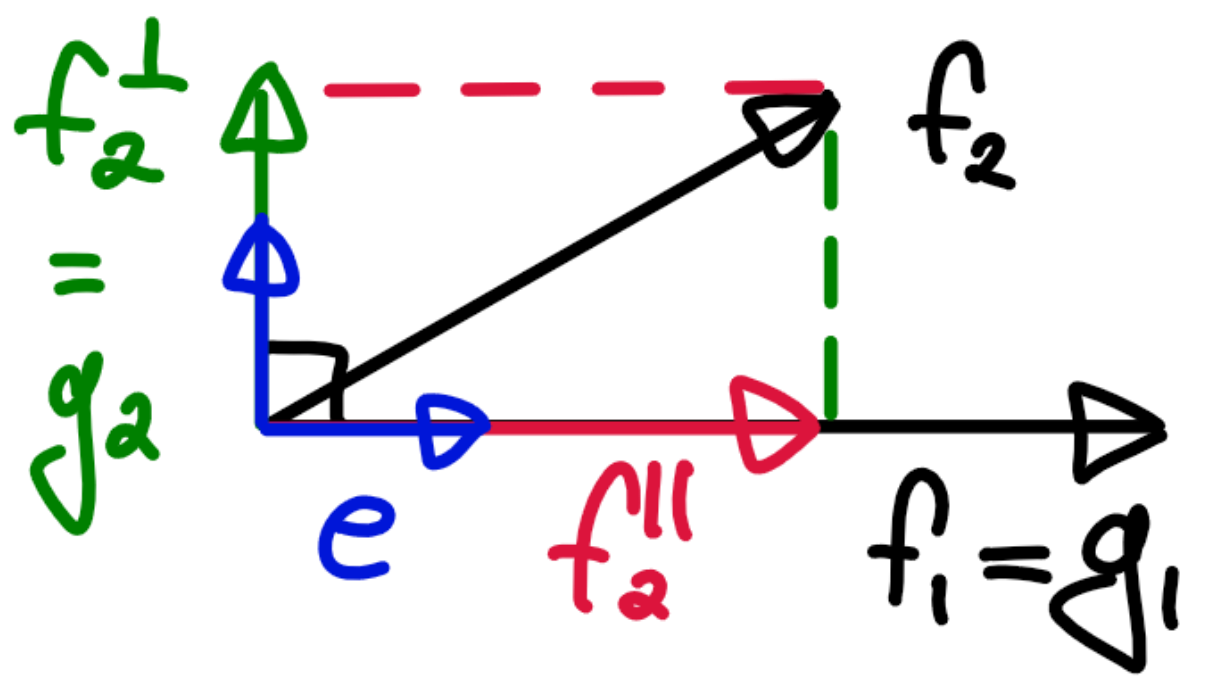
\includegraphics[width=0.25\textwidth]{graphics/12_vectors.png}
\end{figure}

По образовавшемуся из векторов треугольнику $|f_2^\parallel| = |f_2| \cdot \cos(f_2, g_1)$
и из скалярного произведения $(f_2, g_1) = |f_2| \cdot |g_1| \cdot \cos(f_2, g_1)$ получаем:
\[|f_2^\parallel| = \frac{(f_2, g_1)}{|g_1|} \]

Вдоль базисного $g_1$ направим
\textit{\textcolor{BlueViolet}{единичный вектор}} $e = \frac{g_1}{|g_1|}$,
который, взятием $|f_2^\parallel|$ раз, даст вектор $f_2^\parallel$:
\[f_2^\parallel = |f_2^\parallel| \cdot e =
    \frac{(f_2, g_1)}{|g_1|} \cdot \frac{g_1}{|g_1|} \Rightarrow
    f_2^\parallel = \frac{(f_2, g_1)}{(g_1, g_1)} \cdot g_1\]

Тогда $f_2^\perp$ получается из разности векторов $f_2 - f_2^\parallel$,
он и будет вторым вектором ортогонального базиса:
\[g_2 = f_2^\perp = f_2 - \frac{(f_2, g_1)}{(g_1, g_1)} \cdot g_1\]

Аналогично следующий вектор $g_3$ получаем как нормаль к двум предыдущим:
\[g_3 = f_3 - \frac{(f_3, g_1)}{(g_1, g_1)} \cdot g_1 - \frac{(f_3, g_2)}{(g_2, g_2)} \cdot g_2\]\par

Таким образом, формула получения ортогонального базиса имеет вид:
\[g_k = f_k - \sum_{i=1}^{k-1}\frac{(f_k, g_i)}{(g_i, g_i)} \cdot g_i\]
\subsection*{Пример}
\hspace{36pt}
$f_1 = {(1, 3, -2)}^T, f_2 = {(3, 7, -2)}^T$ --- исходный базис.

$\sqsupset g_1 = f_1 = {(1, 3, -2)}^T$;
\hspace{36pt} $g_2 = f_2 - \frac{(f_2, g_1)}{(g_1, g_1)} \cdot g_1$
\[g_2 = {(3, 7, -2)}^T - \frac{3 + 21 + 4}{1 + 9 + 4} \cdot {(1, 3, -2)}^T =
    {(3, 7, -2)}^T - 2 \cdot {(1, 3, -2)}^T = \]
\[ = {(3 - 2, 7 - 6, -2 + 4)}^T = {(1, 1, 2)}^T \]

\underline{Проверка:} $(g_1, g_2)$? $\equiv 0$:\hspace{36pt}
$(g_1, g_2) = 1 + 3 - 4 = 4 - 4 = 0$ --- верно.

\underline{Ответ:} $g_1 = {(1, 3, -2)}^T$, $g_2 = {(1, 1, 2)}^T$ --- ортогональный базис.

\section{Ортогональные матрицы}
\textbf{Опр.} Квадратная матрица $A$ --- ортогональная, если она невырождена и
$A^T = A^{-1} \Leftrightarrow A \cdot A^T = A^T \cdot A = E$:
\[
    \begin{pmatrix}
        a_{11} & a_{12} & \cdots & a_{1n} \\
        a_{21} & a_{22} & \cdots & a_{2n} \\
        \vdots & \vdots & \ddots & \vdots \\
        a_{n1} & a_{n2} & \cdots & a_{nn}
    \end{pmatrix}
    \cdot
    \begin{pmatrix}
        a_{11} & a_{21} & \cdots & a_{n1} \\
        a_{12} & a_{22} & \cdots & a_{n2} \\
        \vdots & \vdots & \ddots & \vdots \\
        a_{1n} & a_{2n} & \cdots & a_{nn}
    \end{pmatrix}
    =
    \begin{pmatrix}
        1      & 0      & \cdots & 0      \\
        0      & 1      & \cdots & 0      \\
        \vdots & \vdots & \ddots & \vdots \\
        0      & 0      & \cdots & 1
    \end{pmatrix}
\]

Строки ортогональной матрицы образуют ортонормированный базис (ОНБ):\\
\hspace*{36pt} $\forall \delta_i\textrm{(строк)}$ верно
$\delta_i \perp \delta_{i+1} \ \Leftrightarrow \ (\delta_i, \delta_{i+1}) = 0$,
при $i = \{1,\ \dots,\ n-1\} \quad \Rightarrow$\\ \hspace*{36pt}
$\delta_1 \cdot \delta_1 = a_{11}^2 + a_{12}^2 +\textrm{\dots}+ a_{1n}^2 = 1$,
т.к. вектор, соответствующий $\delta_1$ не $\perp$ самому себе; \hspace*{36pt}
$\delta_1 \cdot \delta_2 = a_{11}a_{21} + a_{12}a_{22} +\textrm{\dots}+ a_{1n}a_{2n} = 0$,
как у $\perp$ векторов

Аналогично получая подобные выражения для произведения других сочетаний строк, получаем
$\delta_i \cdot \delta_j =
    \begin{cases}
        1, & i = j    \\
        0, & i \neq j
    \end{cases}$
\subsection*{Пример}
\hspace{36pt}
Матрица поворота в $\mathbb{R}^2$:
$ A =
    \begin{pmatrix}
        \cos{\alpha} & -\sin{\alpha} \\
        \sin{\alpha} & \cos{\alpha}
    \end{pmatrix}
    \textrm{,}\quad A^T =
    \begin{pmatrix}
        \cos{\alpha}  & \sin{\alpha} \\
        -\sin{\alpha} & \cos{\alpha}
    \end{pmatrix}$\\
\[
    A \cdot A^T =
    \begin{pmatrix}
        \cos{\alpha}^2 + \sin{\alpha}^2                     &
        \cos{\alpha}\sin{\alpha} - \sin{\alpha}\cos{\alpha}   \\
        \sin{\alpha}\cos{\alpha} - \cos{\alpha}\sin{\alpha} &
        \sin{\alpha}^2 + \cos{\alpha}^2
    \end{pmatrix}
    % ---
    =
    % ---
    \begin{pmatrix}
        1 & 0 \\
        0 & 1
    \end{pmatrix}
    = E
\]
\section{Ортогональные операторы. Связь ортогональности оператора и матрицы оператора}
\subsection*{Ортогональные операторы}
\textbf{Опр.} Линейный оператор $L(x)$ называется ортогнальным (преобразованием),
если он сохраняет скалярное произведение в евклидовом пространстве
$\Leftrightarrow (A(x), A(y)) = (x, y)$.

При таком преобразовании сохраняются:
\begin{enumerate}
    \item длины (нормы) векторов
          \[|(A(x), A(x))| = |(x, x)| \Rightarrow |A(x)| = |x|\]
    \item углы между ними
          \[\cos{\angle\bigl(A(x), A(y)\bigr)} =
              \frac{(A(x), A(y))}{|A(x)||A(y)|} =
              \frac{(x, y)}{|x||y|} = \cos{\angle\bigl(x, y\bigr)}\]
\end{enumerate}

\textbf{$(!)$} 1 $\Rightarrow$ 2:
\[(x+y, x+y) = |x+y|^2 = |x|^2 + |y|^2 + 2xy = (x, x) + (y, y) + 2(x, y) \Rightarrow \]
\[ \Rightarrow 2(x, y) = (x+y, x+y) - (x, x) - (y, y)\]
-- векторы правой части сохраняют норму (из 1) $\Rightarrow$
в правой части сохраняется скалярное произведение: $(A(x), A(y)) = (x, y)$.

Применив формулу скалярного произведения получим 2:
\[ (A(x), A(y)) = |A(x)|\cdot|A(y)|\cdot\cos{\bigl(A(x), A(y)\bigr)} \Rightarrow \]
\[ \Rightarrow \cos{\angle\bigl(A(x), A(y)\bigr)} = \frac{(A(x), A(y))}{|A(x)||A(y)|} =
    \frac{(x, y)}{|x||y|} = \cos{\angle\bigl(x, y\bigr)} \]

Ч.т.д.

Перечисленные свойства ортогонального оператора
характеризуют его как обобщение понятия движения
для n-мерного пространства.
\subsection*{Связь ортогональности оператора и матрицы оператора}
\hspace{36pt}
Если в ОНБ матрица линейного оператора ортогональна, то сам оператор также ортогонален.

Для ОНБ верно $(x, y) = x^Ty$, а для ортогональной матрицы $AA^T = E$ $(A^T = A^{-1})$.\\
Тогда $(A(x), A(y)) = x^T A^T Ay = x^T Ey = x^Ty = (x,y)$ ---
выполняется сохранение скалярного произведения $\Rightarrow$ оператор ортогональный.

Обратное тоже верно: $\forall x, y: x^Ty = x^TA^TAy \Rightarrow
    \exists\ x = (0, \dots, 0,\ 1,\ 0, \dots, 0)^T$ с 1 на месте $i$,
$\exists\ y = (0, \dots, 0,\ 1,\ 0, \dots, 0)^T$ с 1 на месте $j$;
$(AA^T)_{ij} = \delta_{ij} =
    \begin{cases}
        1, & i = j    \\
        0, & i \neq j
    \end{cases}$
--- условие ортогональности матрицы выполняется.

\section{Инвариантные подпространства}
\subsection{Определение:}

Подпространство U линейного пространства L называется инвариантным относительно действия линейного оператора A, если $A(U)  \subset  L$.\\
Иными словами, действие оператора на инвариантном подпространстве не выводит за пределы этого подпространства.\\\\
\subsection{Примеры:}
\begin{itemize}
    \item ker $A$
    \item Im $A$
    \item $X(A,\lambda)$ - Множество всех собственных векторов оператора A для собственного числа $\lambda$
\end{itemize}
Рассмотрим проекцию трёхмерного пространства на плоскость YOZ.\\
Тогда инвариантными подпространствами являются:
\begin{itemize}
    \item плоскость YOZ
    \item каждая прямая в плоскости YOZ
    \item прямая OX
    \item нулевой вектор
    \item всё пространство
\end{itemize}
Конечно, нулевой вектор и всё пространство являются тривиальными примерами инвариантных подпространств.

\section{Сопряжённый оператор. Самосопряжённый оператор.}
\subsection{Сопряжённый оператор. Определение:}
Пусть A(x) - линейный оператор на евклидовом пространстве L.\\
Тогда оператор A* называют сопряжённым к A, если для каждой пары векторов выполнено равенство (A(x), y) = (x, A*(y))\\
Если А - матрица оператора A  в ортонормированном базисе, то матрица оператора A* равна матрице $A^T$, транспонированной к A.\\
В самом деле,(A$(x)^{T}$, y) = $x^T$$A^T$y = xA*y для всех столбцов координат x, y. \\
    Следовательно, $A* = A^T$

    \subsection{Самосопряжённый оператор. Определение:}
    Линейный оператор A на евклидовом пространстве называется самосопряжённым, если $<A(x), y)> = <x, A(y)>$

    \subsection{Примеры:}
    \begin{itemize}
        \item Тождественный оператор

              \quad Справа и слева - скалярное произведение векторов
        \item Гомотетия с коэффициентом t(вещественное число)

              \quad Справа и слева - скалярное произведение векторов, умноженное на t
        \item Проекция на плоскость в трёхмерном евклидовом пространстве с обычным скалярным произведением.

              \quad Пусть x = $x_1$ + $x_2$, $x_1$ - проекция на нормаль, $x_2$ - проекция на плоскость.

              \quad y = $y_1$ + $y_2$, $y_1$ - проекция на нормаль, $y_2$ - проекция на плоскость.

              \quad Тогда $<A(x), y> = <A(x_1 + x_2), y> = <x_2, y_1 + y_2> = <x_2, y_2>$

              \quad Тогда $<x, A(y)> = <(x_1 + x_2), A(y_1 + y_2)> = <x_1 + x_2, y_2> = <x_2, y_2>$

              \quad Следовательно, $<A(x), y> = <x, A(y)>$
    \end{itemize}

    \subsection{Свойство собственных векторов самосопряжённого оператора:}
    Собственные векторы самосопряжённого оператора, соответствующие разным собственным числам, ортогональны.

    \subsubsection{Доказательство:}

    Пусть $\lambda, \mu$ - собственные числа самосопряжённого оператора A.

    Тогда $A(x) = \lambda x, A(y) = \mu y$.

    \[
        \lambda \not \equiv \mu
    \]
    \[
        \langle A(x), y \rangle = \langle x, A(y) \rangle
    \]
    \[
        \lambda \langle x, y\rangle = \mu \langle x, y\rangle
    \]
    \[
        \langle \lambda - \mu\rangle\langle x, y\rangle = 0
    \]

    Поскольку ($\lambda - \mu \not\equiv 0$), получим $\langle x, y\rangle = 0$

    Следовательно, x ортогонально y.

    \setcounter{section}{17}
    \section{Метод Лагранжа (выделение полных квадратов)}
    Этот метод удобен для приведения к диагональному виду квадратичной формы, если собственные числа иррациональные. В общем случае:
    \[
        \sum_{i,j=1}^n a_{ij}x_ix_j = a_{11}x_1^2 + a_{12}x_1x_2 + ...
    \]
    Тогда алгоритм диагонализации:
    \begin{enumerate}
        \item Разделить на $a_{11}$ (или вынести за скобку)
        \item Рассмотреть все слагаемые, содержащие $x_1$
        \item Вместе с выражением $x_1^2$ выделить полный квадрат (возможно, прибавляя и вычитая квадраты остальных $x_i$), воспользовавшись формулой:
              \[
                  (\sum_{i = 1}^n a_i)^2 = \sum_{i = 1}^na_i^2 + 2\sum_{i,j=1, i<j}^na_ia_j
              \]
        \item Сделать замену переменной $\displaystyle y_1 = x_1 + \sum_{i=2}^nt_ix_i$
        \item В итоге квадратичная форма примет вид:
              \[
                  y_1^2 + \sum_{i,j=2}^na_{ij}x_ix_j
              \]
              где $\displaystyle \sum_{i,j=2}^na_{ij}x_ix_j$ — квадратичная форма с меньшим количеством слагаемых. После этого остаётся лишь повторять алгоритм до того момента, пока квадратичная форма не примет вид:
              \[
                  \sum_{i=1}^nb_iy_i^2
              \]
    \end{enumerate}

    Если в квадратичной форме все коэффициенты на главной диагонали равны $0$ ($a_{ii} = 0$, остались только слагаемые вида $a_{ij}x_ix_j, i \neq j$) можно воспользоваться следующей заменой:
    \[
        \begin{cases}
            x_i = x_i' - x_j' \\
            x_j = x_i' + x_j'
        \end{cases}
    \]

    Простейший пример подобного:
    \[
        x_1x_2 = (x_1' - x_2')(x_1' + x_2') = {x_1'}^2 - {x_2}^2
    \]

    В итоге форма также придёт к диагональному виду

    \subsection{Пример}
    \[
        \begin{array}{l}
            4x_1^2 + x_2^2 + 3x_3^2 - 4x_1x_2 + 2x_1x_3 + 2x_2x_3                                                                                           \\
            \text{Поделим на } a_1 = 4                                                                                                                      \\
            x_1^2 + \dfrac{1}{4}x_2^2 + \dfrac{3}{4}x_3^2 - x_1x_2 + \dfrac{1}{2}x_1x_3 + \dfrac{1}{2}x_2x_3                                                \\
            \text{Выделим полный квадрат}                                                                                                                   \\
            (x_1 - \dfrac{1}{2}x_2 + \dfrac{1}{4}x_3)^2 = x_1^2 + \dfrac{1}{4}x_2^2 + \dfrac{1}{16}x_3^2 - x_1x_2 + \dfrac{1}{2}x_1x_3 - \dfrac{1}{4}x_2x_3 \\
            \text{Сделаем замену } y_1 = x_1 - \dfrac{1}{2}x_2 + \dfrac{1}{4}x_3                                                                            \\
            y_1^2 + \dfrac{11}{16}x_3^2 + \dfrac{3}{4}x_2x_3                                                                                                \\
            \text{Поделим на } \dfrac{11}{16}                                                                                                               \\
            \dfrac{16}{11}y_1^2 + x_3^2 + \dfrac{12}{11}x_2x_3                                                                                              \\
            \text{Выделим полный квадрат}                                                                                                                   \\
            (x_3 + \dfrac{6}{11}x_2)^2 = x_3^2 + \dfrac{36}{121}x_2^2 + \dfrac{12}{11}x_2x_3                                                                \\
            \text{Сделаем замену } y_2 = x_3 + \dfrac{6}{11}x_2                                                                                             \\
            \dfrac{16}{11}y_1^2 + y_2^2 - \dfrac{36}{121}x_2^2                                                                                              \\
            \text{Сделаем замену } y_3 = x_2                                                                                                                \\
            \dfrac{16}{11}y_1^2 + y_2^2 - \dfrac{36}{121}y_3^2 \text{ — диагональный вид}                                                                   \\
            \text{Сделав ещё одну замену } z_1 = \dfrac{4y_1}{\sqrt{11}}, z_2 = y_2, z_3 = \dfrac{6y_3}{11} \text{ можно прийти к каноническому виду}       \\
            z_1^2 + z_2^2 - z_3^2 \text{ — канонический вид}
        \end{array}
    \]

    \section{Закон инерции квадратичной формы}
    Закон инерции квадратичных форм гласит: число положительных, отрицательных и нулевых диагональных коэффициентов квадратичной формы не зависит от невырожденного преобразования, с помощью которого квадатичная форма приводится к диагональному виду.

    Число положительных диагональных коэффициентов квадратичной формы называется \textbf{положительным индексом инерции} квадратичной формы. Число отрицательных диагональных коэффициентов квадратичной формы называется \textbf{отрицательным индексом инерции} квадратичной формы. Разность между положительным и отрицательным индексами квадратичной формы называется \textbf{сигнатурой} квадратичной формы. Число ненулевых диагональных коэффициентов называется \textbf{рангом} квадратичной формы.

    \subsection{Доказательство}
    Пусть закон инерции не работает. Тогда разными преобразованиями одной квадратичной формы можно получить две формы с различным числом положительных, отрицательных и нулевых диагональных коэффициентов.
    \[
        F(x) = \sum^n_{i,j=1}a_{ij}x_ix_j
    \]

    Приведём к двум диагональным видам ($\forall \alpha, b > 0$):
    \[
        F(x) = \sum^k_{i=1}\alpha_{i}y_i^2 - \sum^n_{i=k + 1}\alpha_{i}y_i^2
        \\
        F(x) = \sum_{i=1}^lb_iz_i^2 - \sum_{i = l + 1}^nb_iz_i^2
    \]

    Так как это одна и та же форма, то справедливо равенство:
    \[
        \sum^k_{i=1}\alpha_{i}y_i^2 - \sum^n_{i=k + 1}\alpha_{i}y_i^2 = \sum_{i=1}^lb_iz_i^2 - \sum_{i = l + 1}^nb_iz_i^2
    \]

    Пусть $k > l$, т. е. количества не совпали. Тогда найдётся такой ненулевой набор $x_1, ..., x_n$, что:
    \[
        \left.\begin{cases}
            y_{k + 1} = \sum_{i = 1}^{n}c_{k + 1,i}x_i = 0 \\
            y_{k + 2} = \sum_{i = 1}^{n}c_{k + 2,i}x_i = 0 \\
            \vdots                                         \\
            y_{n} = \sum_{i = 1}^{n}c_{n,i}x_i = 0         \\
            z_{1} = \sum_{i = 1}^{n}d_{1,i}x_i = 0         \\
            z_{2} = \sum_{i = 1}^{n}d_{2,i}x_i = 0         \\
            \vdots                                         \\
            z_{l} = \sum_{i = 1}^{l}d_{l,i}x_i = 0         \\
        \end{cases}\right|
        \text{ — СЛУ с $n$ неизвестных ($x_1, ..., x_n$)}
    \]

    Количество уравнений: $(n - k) + l = n - (k - l) < n$, где $n - k$ — количество уравнений для $y$, $l$ — количество уравнений для $z$, $k - l > 0$ по условию.

    СЛУ однородное, содержит $n$ неизвестных и $n - k + l < n$ уравнений, следовательно найдётся ненулевое решение. Обозначим его за $x_1^*, ..., x_n^*$

    Подставим набор в равенство квадратичных форм и оно сократится до:
    \[
        \sum^k_{i=1}\alpha_{i}y_i^2 = -\sum_{i = l + 1}^nb_iz_i^2
    \]

    Для того, чтобы $y_{1}, ..., y_k = 0$ и $z_{l + 1}, ..., z_n = 0$ необходимо, чтобы все $x_i^* = 0$, но набор был взят ненулевой, следовательно условие $k > l$ приводит к противоречию. Аналогично и для $k < l$.

    \subsection{Пример}
    Приведём квадратичную форму $x_1x_2 + 2x_1x_3 + 4x_2x_3$ к диагональному виду:
    \[
        \begin{cases}
            y_1 = \dfrac{1}{2}x_1 + \dfrac{1}{2}x_2 + 3x_3 \\
            y_2 = -x_1 + x_2 - 2x_3                        \\
            y_3 = x_3                                      \\
        \end{cases} \Rightarrow
        \begin{cases}
            x_1 = y_1 - \dfrac{1}{2}y_2 - 4y_3 \\
            x_2 = y_1 + \dfrac{1}{2}y_2 - 2y_3 \\
            x_3 = y_3                          \\
        \end{cases}
    \]
    \[
        \begin{cases}
            z_1 = \dfrac{1}{2}x_1 + \dfrac{1}{2}x_2 + 3x_3 \\
            z_2 = -\dfrac{1}{2}x_1 + \dfrac{1}{2}x_2 - x_3 \\
            z_3 = 2x_3                                     \\
        \end{cases} \Rightarrow
        \begin{cases}
            x_1 = z_1 - z_2 - 2z_3 \\
            x_2 = z_1 + z_2 - z_3  \\
            x_3 = \dfrac{1}{2}z_3  \\
        \end{cases}
    \]
    Получим два диагональных вида:
    \[
        y_1^2 - \dfrac{1}{4}y_2^2 - 8y_3^2 \\ z_1^2 - z_2^2 - 2z_3^2
    \]
    При этом можно заметить, что оба вида имеют одинаковое количество положительных и отрицательных коэффициентов.

    \section{Примеры приведения уравнения кривой второго порядка и поверхности второго порядка к канонической форме}
    Выбор метода зависит от поставленной задачи. Вычисление с помощью собственных векторов и ортонормированного базиса позволяет применить движение плоскости или пространства и решить вычислительные задачи.

    Преобразование методом Лагранжа удобнее применить, если собственные числа иррациональны. При этом некоторые величины (например, координаты центра при его наличии) найти удастся, но некоторые другие (например, координаты фокусов) не удастся. С применением закона инерции квадратичной формы можно определить тип кривой или поверхности, но вычислительные возможности ниже. Однако вычислений может потребоваться меньше.

    \subsection{Приведение уравнения кривой второго порядка $11x^2 + 19y^2 + 6xy - 28x - 44y = 14$ к каноническому виду}
    \[
        A = \begin{pmatrix}
            11 & 3  \\
            3  & 19
        \end{pmatrix}
        \\
        B = \begin{pmatrix}
            11 - \lambda & 3            \\
            3            & 19 - \lambda
        \end{pmatrix}
    \]
    \[
        |B| = \lambda^2 - 30\lambda + 200 = 0
        \\ \lambda_{1, 2} = 10; 20
    \]
    \[
        \lambda = 20:
        \begin{pmatrix}
            -9 & 3  \\
            3  & -1
        \end{pmatrix}
        \Rightarrow
        3x_1 = x_2
        \Rightarrow
        e_1 = t\begin{pmatrix}1 \\ 3\end{pmatrix}
    \]
    \[
        \lambda = 10:
        \begin{pmatrix}
            1 & 3 \\
            3 & 9
        \end{pmatrix}
        \Rightarrow
        x_1 = -3x_2
        \Rightarrow
        e_2  = t\begin{pmatrix}3 \\ -1\end{pmatrix}
    \]
    \[
        C = \dfrac{1}{\sqrt{10}}\begin{pmatrix}
            1 & 3  \\
            3 & -1
        \end{pmatrix} \text{ — ортогональная}
        \Rightarrow
        C^{-1} = C^T
    \]
    \[
        C^{-1} = C^T, C^T = C \Rightarrow C^{-1} = C
    \]
    \[
        \begin{cases}
            x = \dfrac{x' + 3y'}{\sqrt{10}} \\
            y = \dfrac{3x' - y'}{\sqrt{10}}
        \end{cases} \\
        \begin{cases}
            x' = \dfrac{x + 3y}{\sqrt{10}} \\
            y' = \dfrac{3x - y}{\sqrt{10}}
        \end{cases}
    \]
    \[
        \dfrac{11(x' + 3y')^2 + 19(3x' - y')^2 + 6(x' + 3y')(3x' - y')}{10} - \dfrac{28(x' + 3y') + 44(3x' - y')}{\sqrt{10}} = 14
    \]
    \[
        20{x'}^2 + 10{y'}^2 - 16\sqrt{10}x' - 4\sqrt{10}y' = 14
    \]
    \[
        20(x' - \dfrac{4}{\sqrt{10}})^2 - 32 + 10{y'}^2 - 4\sqrt{10}y' = 14
    \]
    \[
        20(x' - \dfrac{4}{\sqrt{10}})^2 - 32 + 10(y' - \dfrac{2}{\sqrt{10}})^2 - 4 = 14
    \]
    \[
        20(x' - \dfrac{4}{\sqrt{10}})^2 + 10(y' - \dfrac{2}{\sqrt{10}})^2 = 50 \\ |:50
    \]
    \[
        \dfrac{x' - \dfrac{4}{\sqrt{10}}}{\sqrt{\dfrac{5}{2}}}^2 + \dfrac{y' - \dfrac{2}{\sqrt{10}}}{\sqrt{5}}^2 = 1
    \]
    \[
        \begin{cases}
            x'' = y' - \dfrac{2}{\sqrt{10}} \\
            y'' = x' - \dfrac{4}{\sqrt{10}} \\
        \end{cases}
        \\
        \begin{cases}
            x' = y'' + \dfrac{4}{\sqrt{10}} \\
            y' = x'' + \dfrac{2}{\sqrt{10}} \\
        \end{cases}
    \]
    \[
        \dfrac{x''}{\sqrt{5}}^2 + \dfrac{y''}{\sqrt{\dfrac{5}{2}}}^2 = 1
    \]
    \subsection{Приведение поверхности второго порядка $4x^2 + y^2 + 3z^2 - 4xy + 2xz + 2yz - 2x + 4y + 2z = 0$ к канонической форме}
    \[
        (2x - y - z)^2 = 4x^2 + y^2 + z^2 - 4xy - 4xz + 2yz
    \]
    \[
        (2x - y + z)^2 + 2(z^2 + 3xz) - 2x + 4y + 2z = 0
    \]
    \[
        2(z + \dfrac{3}{2}x)^2 = 2z^2 + 6xz + \dfrac{9}{2}x^2
    \]
    \[
        (2x - y - z)^2 + 2(z + \dfrac{3}{2}x)^2 - \dfrac{9}{2}x^2 - 2x + 4y + 2z = 0
    \]
    \[
        \begin{cases}
            x' = 2x - y - z        \\
            y' = z + \dfrac{3}{2}x \\
            z' = x
        \end{cases}
        \\
        \begin{cases}
            x = z'                        \\
            y = -x' - y' + \dfrac{7}{2}z' \\
            z = y' - \dfrac{3}{2}z'
        \end{cases}
    \]
    \[
        {x'}^2 + 2{y'}^2 - \dfrac{9}{2}{z'}^2 - 2z' - 4x' - 4y' + 14z' + 2y' - 3z' = 0
    \]
    \[
        {x'}^2 + 2{y'}^2 - \dfrac{9}{2}{z'}^2 - 4x' - 2y' + 9z' = 0
    \]
    \[
        (x' - 2)^2 - 4 + 2\left(y' - \dfrac{1}{2}\right)^2 - \dfrac{1}{2} - \dfrac{9}{2}\left(z' - 1\right)^2 + \dfrac{9}{2} = 0
    \]
    \[
        (x' - 2)^2 + 2\left(y' - \dfrac{1}{2}\right)^2 - \dfrac{9}{2}\left(z' - 1\right)^2 = 0
    \]
    \[
        \begin{cases}
            x'' = x' - 2            \\
            y'' = y' - \dfrac{1}{2} \\
            z'' = z' - 1
        \end{cases}
        \\
        \begin{cases}
            x' = x'' + 2            \\
            y' = y'' + \dfrac{1}{2} \\
            z' = z'' + 1
        \end{cases}
    \]
    \[
        {x''}^2 + \left(\dfrac{y''}{\frac{1}{\sqrt{2}}}\right)^2 - \left(\dfrac{z''}{\frac{\sqrt{2}}{3}}\right)^2 = 0
    \]

    \section{22. Критерий Сильвестра}
    \begin{itemize}
        \item Квадратичная форма является
              \textit{положительно определенной} (т.е.
              принимает только положительные значения
              на ненулевых векторах) тогда и только тогда,
              когда все верхние угловые миноры положительны.
        \item Квадратичная форма является
              \textit{отрицательно определенной} (т.е.
              принимает только отрицательные значения
              на ненулевых векторах) тогда и только тогда,
              когда все миноры знакопеременны, начиная с "$-$".
    \end{itemize}
    \subsection{Примечания:}

    \begin{enumerate}
        \item Если определитель матрицы квадратичной формы не равен 0 и цепочка миноров не отвечает ни требованиям для положительной определенности, ни требованиям для отрицательной определенности,то форма на ненулевых векторах принимает значения разных знаков, и такая квадратичная форма будет называется  \textit{неопределенной} (или формой общего вида).
        \item Если определитель матрицы квадратичной формы равен 0, то знаки миноров не несут информации про значения формы.
    \end{enumerate}

    \subsection{Доказательство необходимости для случая положительной определенности:}

    Докажем, что если форма положительно определена, то все левые верхние угловые миноры положительны:

    Пусть квадратичная форма имеет вид $F(x) = \sum\limits_{i,j=0}^n a_{ij} x_{i} x_{j}$

    Существует приведение к каноническому виду - невырожденное преобразование с матрицей C:
$A = C^{T}DC, D$ - диагональная матрица, элементы на диагонали > 0

    Тогда det $A = det C^{T}DC = det C^{T} \cdot det D \cdot det C = det D \cdot (detC)^{2}$ => матрица С невырожденная

    Докажем, что все верхние угловые миноры > 0:

    Рассмотрим минор размером k х k. Рассмотрим вектор, в котором первые k элементов равны 1, остальные равны 0. Для таких наборов квадратичная форма положительно определена, поэтому определитель минора размером k х k положителен.

    \subsection{Примеры:}

    \begin{enumerate}
        \item $x^2_{1} + 26x^2_{2} + 10x_{1}x_{3}$
              \[
                  A = \left(
                  \begin{array}{rrr}
                          1 & 5  \\
                          5 & 26
                      \end{array}
                  \right)
              \]
              $det A = 26 - 25 = 1 > 0$; верхний минор размером 1х1 > 0 => положительно определенная - по критерию Сильвестра.

        \item $-x^2_{1} - 4x^2_{2} + 2x_{1}x_{2}$

              \[
                  A = \left(
                  \begin{array}{rrr}
                          -1 & 1  \\
                          1  & -4
                      \end{array}
                  \right)
              \]
              $det A = 4 - 2 = 2 > 0$; верхний минор размером 1х1 < 0 => отрицательно определенная - по критерию Сильвестра.
        \item $x^2_{1} - 15x^2_{2} + 4x_{1}x_{2} - 2x_{1} x_{3} + 6x_{2} x_{3}$

              \[A = \left(
                  \begin{array}{rrr}
                          1  & 2   & -1 \\
                          2  & -15 & 3  \\
                          -1 & 3   & 0
                      \end{array}
                  \right)\]

              Верхний минор размером 1х1 положителен, определитель минора 2х2 отрицателен, det A = -6 $\neq$ 0 => форма не является ни положительно определенной, ни отрицательно определенной => неопределенная - по критерию Сильвестра.
    \end{enumerate}

    \setcounter{section}{24}
    \section{Отображение групп, гомоморфизм.}
    \subsection{Определение}
$G_1 \rightarrow G_2$, где $(G_1,\cdot)$ - группа, а $(G_2,\times)$ - группа, называется гомоморфизмом, если он сохраняет групповую структуру: $\forall a,b\in G_1: \varphi(a\cdot b)=\varphi(a)\times\varphi(b)$, $\varphi(a),\varphi(b)\in G_2$. Если, кроме того, $\varphi$ является взаимно-однозначным, то $\varphi$ называют изоморфизмом (биекцией).

    Если $\varphi:G_1\rightarrow G_2$ -- биекция, то $\varphi$ -- изоморфизм.

    Если для двух групп существует изоморфизм, группы называют изоморфными.

    Если образом $\varphi$ является вся группа $G_2$, то $\varphi$ называют эпиморфизмом (сюръекцией).

    Если гомоморфизм имеет вид $\varphi(G_1)=G_2$, то он называется сюръекцией.

    Если для каждых двух различных элементов $a,b\in G_1$ при действии $\varphi$ различаются их образы, то $\varphi$ называют мономорфизмом или же (инъекцией).

    Если $\varphi(a)=\varphi(b) \Rightarrow a=b$, то гомоморфизм называется инъекцией.

    Гомоморфизм группы на себя называется автоморфизмом. Простейший пример автоморфизма - тождественный автоморфизм при котором $f(x) = x$

    \subsection{Примеры гомоморфизма:}
    \begin{enumerate}
        \item Проекция трехмерных векторов на плоскость. Проекция суммы равна сумме проекций.

        \item Нахождение остатка от деления на 9 – гомоморфизм между группами: $(G_1,\cdot)$ целые числа с умножением, $(G_2,\times)$ --- множество (0,1,2,3,4,5,6,7,8) с умножением, при котором результат произведения заменяется остатком от деления на 9.
    \end{enumerate}

    \section{Изоморфизм}
    \subsection{Определение}
    Изоморфизм --- это биективный гомоморфизм.\\Если $f:G_1\rightarrow G_2$ --- биекция, то $f$ --- изоморфизм.

    \subsection{Проверка изоморфности:}
    \begin{enumerate}
        \item Найти свойство, которое есть у одной $G$, но отсутствует у другой.
        \item Если не нашлось, то построить изоморфизм.
    \end{enumerate}
    \subsection{Примеры}
    \begin{enumerate}
        \item \textbf{(Изоморфные группы)} Операция сопряжения в множестве комплексных чисел является изоморфизмом и относительно сложения, и относительно умножения. Это отображение взаимно-однозначно из соображений симметрии. Проверим выполнение условия на гомоморфизм для сложения:
              \[
                  z_1 = a_1 + b_1i  и z_2 = a_2 + b_2i
              \]
              \[
                  f(z_1+z_2) = (\overline{(a_1 + b_1i + a_2 + b_2i)}) = a_1 + a_2 - (b_1 + b_2)i = f(z_1) - f(z_2)
              \]
              И проверим условие на гомоморфизм для умножения:
              \[
                  f(z_1*z_2)=(\overline{(a_1+b_1i)*(a_2+b_2i)}=a_1a_2-(b_1b_2)+(a_1b_2+a_2b_1)i=f(z_1)*f(z_2)
              \]
        \item Мн-ч степени ≤ 2 со сложением. Гомоморфизм - взаимно-однозначное соответствие коэффициентов мн-ч. 2.
        \item Трёхмерные векторы со сложением. Гомоморфизм - взаимно-однозначное соответствие координат вектора. Доказательство изоморфности проводится построением изоморфизма.
        \item $(R^+,\cdot)$ и $(R,+)$ - – группы. В качестве изоморфизма возьмем: $f(x) = \ln(x)$. Отображение взаимно-однозначное.
              Условие гомоморфизма выполняется: $(a · b) = \ln(a · b) = \ln(a) + \ln(b) = f(a) + f(b)$

        \item $(Q^+,\cdot)$ и $(Q,+)$ – группы. В рациональных числах можно делить на 2, но не всегда можно извлечь квадратный корень.

              Пусть из $(Q,+)$ в $(Q^+, \cdot)$  построен изоморфизм $f(x)$. Обратное $f(x)$ отображение --- $g(x)$. Найдётся такое рациональное число $a$, что $a + a = g(2)$.
              Тогда применим к этому равенству отображение $f(x)$ и получим $f(a)f(a) = 2$. Это противоречит иррациональности $\sqrt{2}$. Следовательно,изоморфизма нет.
    \end{enumerate}

    \section{Смежные классы}
    \subsection{Определение}
    Пусть $G$ --- группа, $H$ --- подгруппа. Введем отношение $\sim$ на $G$: $a\sim b \Leftrightarrow a^{-1}b\in H$, где $a^{-1}$ ---
    мультипликативная запись действия, т.е. действие в виде произведения.

    Определение: отношение на множестве $G$ --- это подмножество декартового квадрата $G\times G$. Т.е. для каждых двух элементов можно сказать, находятся ли они в этом отношении. Отношение $a\sim b \Leftrightarrow a^{-1}b\in H$ обладает свойствами:

    \subsection{Свойства}
    \begin{itemize}
        \item Рефлексивность: $\forall a: a\sim a$, т.е. $a^{-1}a=e$.
        \item Симметричность: $a\sim b \Rightarrow b\sim a$.
        \item Транзитивность: $a\sim b, b\sim c \Rightarrow a\sim c$. \end{itemize}
    \subsection{Обобщение классов вычетов}
    ] у нас есть группа $G=(\mathbb{Z},+)$, $H=(7\mathbb{Z},+)$, тогда два числа лежат в одном классе, когда дают одинаковый остаток от деления на 7. Правый смежный класс $(H_a)$ позволяет определить отношение $a\sim b$.

    Левый смежный класс $({}_aH)$ - для отношения $a\sim b \Leftrightarrow a^{-1}b\in H$.

    Подгруппа $H$ группы $G$ называется нормальной, если для каждого элемента $a$ из $G$ левый смежный класс и правый смежный класс совпадают.

    \subsection{Примеры} G= $(Z,+)$, H= $(7Z,+)$, Тогда два числа лежат в одном классе тогда и только тогда, когда дают одинаковый остаток от деления на 7. Таким образом, смежные классы – обобщение классов вычетов.

    \section{Ядро и образ гомоморфизма}
    \subsection{Определение}
    Пусть $(G_1,\cdot)$ и $(G_2,*)$ - две группы, а $f$ - гомоморфизм из $G_1$ в $G_2$.

    Ядро гомоморфизма $f$, $\operatorname{ker}(f)$, определяется как множество всех $x$ из $G_1$ таких, что $f(x)=e_{G_2}$.

    Образ гомоморфизма $f$, $\operatorname{im}(f)$, определяется как множество всех $y$ из $G_2$ таких, что существует $x$ из $G_1$ такой, что $f(x)=y$. То есть, образ гомоморфизма - это множество всех элементов.

    Докажем, что ядро и образ являются подгруппами относительно соответствующих групп.

    \subsection{Для ядра}

    Замкнутость выполняется, так как если $x_1,x_2\in \operatorname{ker}(f)$, то \\ $f(x_1)=f(x_2)=e_{G_2}$ и $f(x_1\cdot x_2)=f(x_1)*f(x_2)=e_{G_2}*e_{G_2}=e_{G_2}$.

    Ассоциативность выполняется, так как действия происходят в группе.

    Существует нейтральный элемент, так как $f(x\cdot e_{G_1})=f(x)*f(e_{G_1})=f(x)$.

    Существуют обратные элементы, так как если $f(x)=e_{G_2}$, то $e_{G_2}=f(e_{G_1})=f(x\cdot x^{-1})=f(x)*f(x^{-1})=e_{G_2}*f(x^{-1})$, откуда следует, что $f(x^{-1})=e_{G_2}$ и $x^{-1}\in \operatorname{ker}(f)$.

    \subsection{Для образа}

    Замкнутость выполняется, так как если $y_1,y_2\in \operatorname{im}(f)$, то \\$\exists x_1,x_2:f(x_1)=y_1,f(x_2)=y_2$ и $y_1*y_2=f(x_1)*f(x_2)=f(x_1\cdot x_2)\in \operatorname{im}(f)$.

Ассоциативность выполняется, так как действия происходят в группе.

Существует нейтральный элемент, так как $f(e_{G_1})=e_{G_2}$.

Существуют обратные элементы, так как если $y\in \operatorname{im}(f)$, то $\exists x:f(x)=y$, $e_{G_2}=f(x\cdot x^{-1})=f(x)*f(x^{-1})=y*f(x^{-1})$, откуда следует, что $f(x^{-1})\in \operatorname{im}(f)$ и является обратным к $y$.

Гомоморфизм является мономорфизмом (инъекцией) тогда и только тогда, когда его ядро тривиально.

Если $(G_1,\cdot)$ и $(G_2,*)$ - две группы, а $f$ - гомоморфизм из $G_1$ в $G_2$, то $\operatorname{ker}(f)$ тривиально и $f(x_1)=f(x_2)\Rightarrow f(x_1)*(f(x_2))^{-1}=e_{G_2}$.

Значит, $f(x_1\cdot x_2^{-1})=f(x_1)*f(x_2^{-1})=e_{G_2}$, то есть, $\operatorname{ker}(f)$ тривиально, и $x_1=x_2$.

\subsection{Пример}

Две группы $(\mathbb{R}^{+},\cdot)$ и $(\mathbb{R},+)$ с гомоморфизмом $f(x) = \ln(x)$. $\ker(f) = \{1\}$, $\operatorname{Im}(f) = \mathbb{R}$. Гомоморфизм является мономорфизмом (инъекцией) тогда и только тогда, когда его ядро тривиально.

\setcounter{section}{30}
\section{ Изображение множества решений систем дифференциальных уравнений на плоскости.}

Для исследования на устойчивость точки покоя систему двух линейных однородных дифференциальных уравнений с постоянными коэффициентами надо составить характеристическое уравнение. В зависимости от вида и знаков корней, можно определить вид точки покоя.
Пусть система дифференциальных уравнений имеет вид :
\[
    \begin{cases}
        y'=a_{11}x+a_{12}y \\
        x'=a_{21}x+a_{22}y
    \end{cases}
\]
Составим характеристическое уравнение det
$\begin{pmatrix}
        a_{11}-\lambda & a_{12}         \\
        a_{21}         & a_{22}-\lambda
    \end{pmatrix} =0$


Из свойств показательной функции и общей формулы для решения системы дифференциальных
уравнений указанного вида можем сделать такие выводы.
Если характеристическое уравнение имеет два отрицательных вещественных корня (или один
отрицательный корень кратности 2), имеем устойчивый узел, если два положительных вещественных корня
(или один положительный корень кратности 2) – неустойчивый узел, если два вещественных корня разных
знаков – седло.
В случае с комплексными корнями с отрицательной вещественной частью получим устойчивый полюс
(фокус), с положительной вещественной частью – неустойчивый полюс (фокус), с нулевой вещественной
частью – центр

\subsection{Наглядные примеры:}

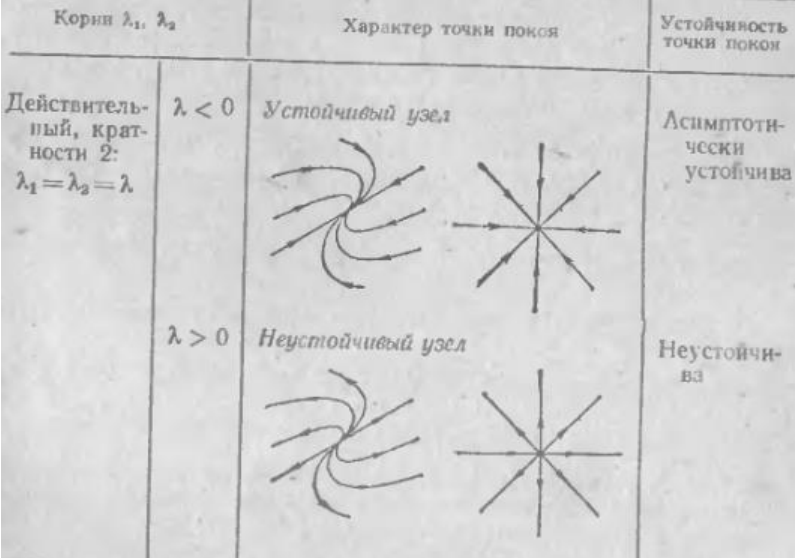
\includegraphics[width=100mm]{graphics/31_de_1.png}

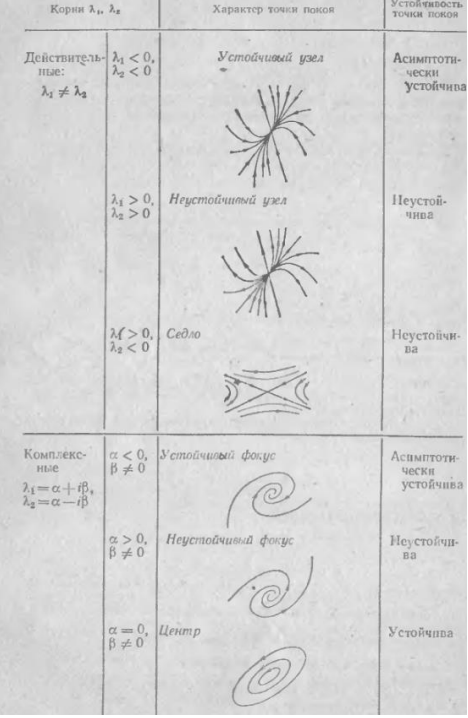
\includegraphics[width=100mm]{graphics/31_de_2.png}

\section{ Решение ДУ с помощью характеристического многочлена (общее и частное)}
Уравнение $a\lambda^2+b\lambda+c=0$ называют характеристическим уравнением дифференциального уравнения ay''+by'+cy=0 Если это уравнение имеет два различных вещественных корня, мы получим
два линейно независимых решения дифференциального уравнения. Для случая с совпадающими корнями
или с комплексными корнями решение придётся несколько модифицировать, эти случаи рассмотрим позже.
Поскольку множество решений дифференциального уравнения второго порядка двумерно (это
теоретический факт, на который ссылаемся без доказательства), то получается, что, решив квадратное
уравнение, мы можем найти два линейно независимых собственных вектора, а их линейная комбинация
даст общее решение для дифференциального уравнения.
Если для дифференциального уравнения заданы значения функции и первой производной в начальной
точке, то можно найти и коэффициенты функции, то есть частное решение. Для этого надо подставить
коэффициенты функции из общего решения в условия на значения функции и производной.

\subsection{Пример}
$y''-5y'+4y=0, y(0)=y'(0) = 1$ (частное решение)
\\
Решим квадратное уравнение $\lambda^2-5\lambda+4=0$
Его корни: 1 и 4.
\\
Общее решение: $C_1e^x+C_2e^{4x}$
\\
Производная от него:  $C_1e^x+4C_2e^{4x}$
\\
Подставим $x = 0$ в условие для функции и производной, получим систему линейных уравнений.
\[
    \begin{cases}
        C_1+C_2=1 \\
        C_1+4C_2=1
    \end{cases}
\]
\begin{align*}
     & C_1 = 1, C_2 = 0                        \\
     & C_1e^x+C_2e^{4x} = 1*e^x+0*e^{4x} = e^x
\end{align*}
Ответ: $e^x$ .

\setcounter{section}{32}
\section{Базис, ЛНЗ}
\subsection{Базис линейного пространства -} порождающая линейно независимая подсистема.

\begin{itemize}
    \item Если каждый элемент пространства можно линейно выразить через некоторую подсистему, то считается, что эта подсистема \textit{порождает} всю систему.

    \item Система элементов линейного пространства $\vec x_{1}, \vec x_{2}, ..., \vec x_{n}$ называется \textit{линейно зависимой}, если существуют числа $a_{1}, a_{2},..., a_{n}$, не все равные 0, такие, что $a_{1}\vec x_{1} + a_{2}\vec x_{2},..., a_{n}\vec x_{n} = \vec 0$, где $\vec 0$ - арифиметический вектор, состоящий из одних нулей (\textit{ноль-вектор}). Если таких коэффициентов не существует, то система называется \textit{линейно независимой}.

\end{itemize}
\subsection{Примеры:}

\begin{enumerate}
    \item Набор из трех векторов, направленных по осям координат в $\mathbb{R}^{3}$:
          (1,0,0), (0,1,1), (0,0,1).

    \item Для пространства многочленов степени не выше $2$: $1, x, x^{2}$.
\end{enumerate}


В векторном простанстве можно выбрать базис и разложить каждый элемент по базису.

\subsection{Переход к новому базису:}

Пусть $e_{1},...,e_{n}$ - прежний базис, $f_{1},...,f_{n}$ - новый базис.

Тогда каждый вектор $f_{k}$ в новом базисе можно выразить через прежний базис:

$f_{k} = \sum\limits_{i=0}^n t_{ik}e_{i}$

Иногда записывают такой переход через матрицу Т - матрицу перехода.

\end{document}